\chapter{Conception Détaillée du Backend et Services Métiers}
\label{chap:backend}

\section{Organisation Modulaire et Motif Application Factory}

Le backend de Perceptra a été conçu selon les règles de l'art du génie logiciel Python moderne. L'application applique rigoureusement le motif \textbf{Application Factory} (\texttt{create\_app}) combiné à l'architecture en \textbf{Blueprints} de Flask~3.x.

Cette organisation garantit l'isolation complète des contextes d'exécution (développement local, suite de tests automatisée sous Pytest et déploiement conteneurisé en production) tout en facilitant l'injection de dépendances et l'isolation des états.

\begin{figure}[H]
\centering
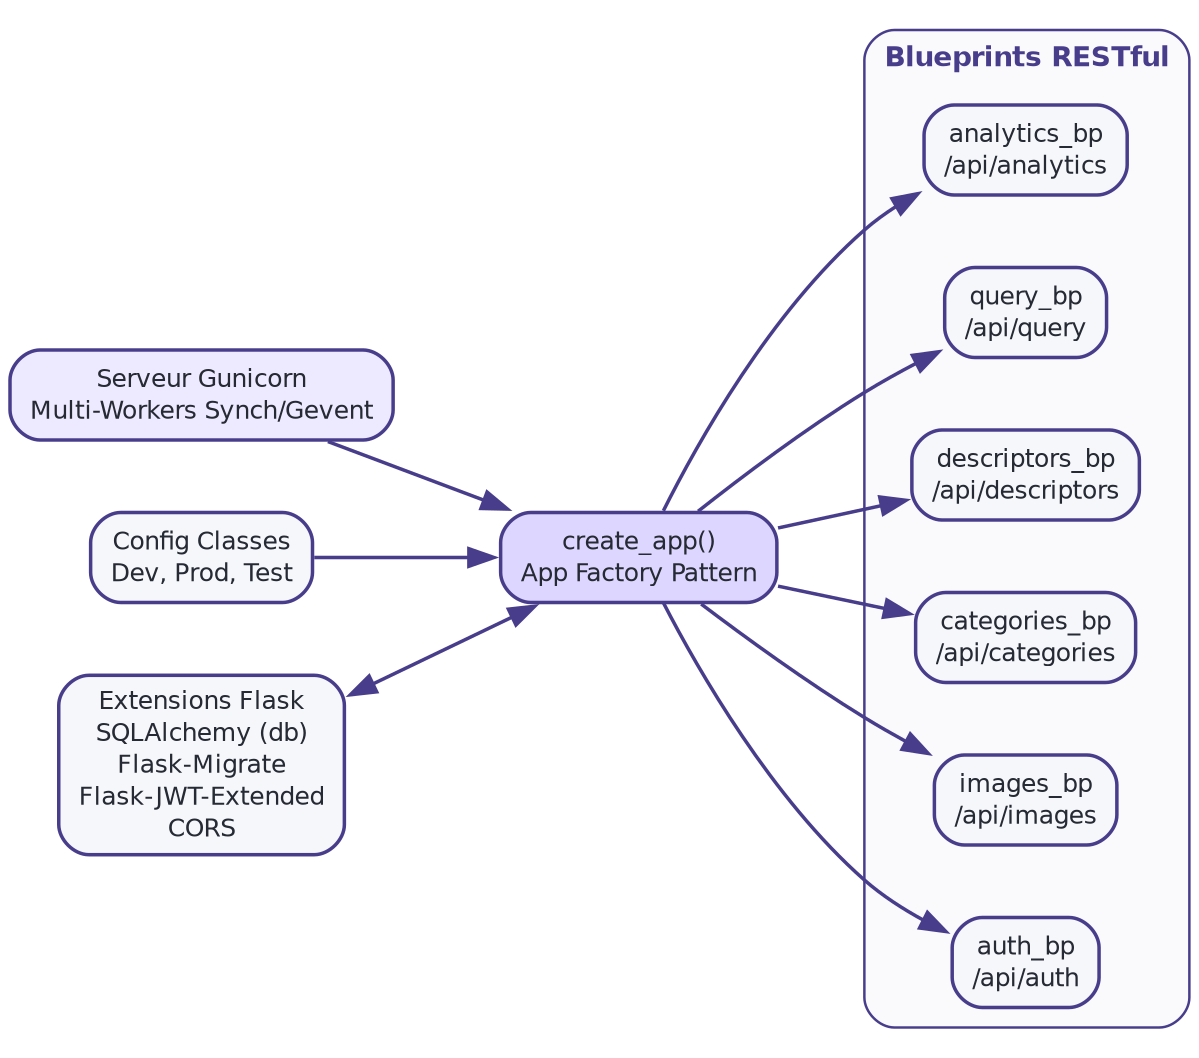
\includegraphics[width=0.76\textwidth]{images/04-architecture-backend-flask.png}
\caption{Architecture modulaire interne du backend Flask et découplage des Blueprints}
\label{fig:backend_flask}
\end{figure}

Le fichier \texttt{src/config.py} structure la hiérarchie des configurations au moyen de classes héritant d'une classe de base commune~: \texttt{DevelopmentConfig} (mode debug, base locale SQLite), \texttt{TestingConfig} (base volatile en mémoire \texttt{sqlite:///:memory:}, désactivation CSRF), et \texttt{ProductionConfig} (sécurité renforcée, support natif PostgreSQL via \texttt{DATABASE\_URL}).

\section{Couche de Routage : Les Blueprints RESTful}

L'ensemble des points d'accès HTTP est distribué dans six Blueprints étanches logés dans le paquet \texttt{src/routes/}~:

\begin{table}[H]
\centering
\rowcolors{2}{LightGray}{white}
\begin{tabularx}{\textwidth}{>{\bfseries}p{3.2cm}p{3.8cm}X}
\toprule
\rowcolor{TableHeader}
\color{white}Blueprint & \color{white}Préfixe d'URL & \color{white}Responsabilités Fonctionnelles \\
\midrule
\texttt{auth\_bp} & \texttt{/api/auth} & Inscription, connexion avec émission de paire de jetons JWT (access/refresh), profil et déconnexion. \\
\texttt{images\_bp} & \texttt{/api/images} & Téléversement unitaire et par lots, listing paginé avec filtres (catégorie, statut, favori), suppression, téléchargement binaire, service de vignettes et retouches d'images. \\
\texttt{categories\_bp} & \texttt{/api/categories} & Création, modification et suppression de catégories hiérarchiques, calcul automatique des chemins et sérialisation en arbre. \\
\texttt{descriptors\_bp} & \texttt{/api/descriptors} & Déclenchement d'extraction, consultation des signatures numériques et données statistiques pour les graphiques de l'UI. \\
\texttt{query\_bp} & \texttt{/api/query} & Moteur de recherche par le contenu : requête simple par image, pondération des descripteurs, et soumission du feedback FRE. \\
\texttt{analytics\_bp} & \texttt{/api/analytics} & Statistiques globales du système, métriques disque, historique auditable des sessions de recherche et profilage de latence. \\
\bottomrule
\end{tabularx}
\caption{Cartographie des contrôleurs Blueprints de l'API REST de Perceptra}
\label{tab:blueprints}
\end{table}

\section{Le Motif « Service Layer » et Découplage Métier}

Pour proscrire tout couplage préjudiciable entre la manipulation des requêtes HTTP et la complexité des algorithmes de calcul, Perceptra implémente le patron architectural \textbf{Service Layer}.

\subsection{1. \texttt{StorageService} : Gestion du Stockage Physique}
Le service \texttt{src/services/storage.py} gère l'écriture, la lecture et la suppression des flux binaires sur le système de fichiers hôte. Ses prérogatives clés incluent~:
\begin{itemize}
    \item \textbf{Calcul d'empreinte SHA-256~:} Avant toute écriture, l'empreinte cryptographique des données binaires est évaluée. Cette somme de contrôle permet d'identifier formellement les doublons et de garantir l'intégrité du stockage.
    \item \textbf{Génération de clés de stockage canoniques~:} Les fichiers sont organisés dans une arborescence chronologique évitant les congestions de répertoires à plat~: \texttt{storage/uploads/YYYY/MM/<uuid>.<ext>}.
    \item \textbf{Service de vignettes (\textit{Thumbnails})~:} Génération automatique de vignettes allégées ($256 \times 256$ pixels, format WebP ou JPEG optimisé) mises en cache sur le disque pour préserver la bande passante.
\end{itemize}

\subsection{2. \texttt{TransformEngine} : Moteur de Retouche Géométrique}
Le module \texttt{src/services/transform\_engine.py} fournit un moteur sans état de transformation géométrique d'images particulièrement robuste. Conçu pour préserver l'image originale intacte (\textit{non-destructive editing}), il génère une nouvelle entité image fille référençant l'image parente via la clé étrangère \texttt{parent\_image\_id}. Les transformations supportées couvrent~:
\begin{itemize}
    \item \textbf{Recadrage (\textit{Crop})~:} Découpage précis selon une boîte englobante $(x, y, w, h)$ avec validation géométrique stricte.
    \item \textbf{Redimensionnement (\textit{Resize})~:} Rééchelonnement avec choix de l'interpolation (LANCZOS pour la fidélité, INTER\_AREA d'OpenCV pour les réductions d'échelle évitant les artefacts de moirage).
    \item \textbf{Rotations et Retournements~:} Rotations orthogonales ($90^\circ, 180^\circ, 270^\circ$) ou continues selon un angle arbitraire $\theta \in [-360^\circ, 360^\circ]$ avec calcul trigonométrique de l'ajustement du cadre pour éliminer tout rognage involontaire.
    \item \textbf{Transformations Affines Généralisées~:} Application d'une matrice affine de transformation $2 \times 3$ combinant homothétie, cisaillement (\textit{shear}) et translation~:
    \begin{equation}
    \begin{bmatrix} x' \\ y' \end{bmatrix} = \begin{bmatrix} a & b \\ d & e \end{bmatrix} \begin{bmatrix} x \\ y \end{bmatrix} + \begin{bmatrix} c \\ f \end{bmatrix}
    \end{equation}
    \item \textbf{Ajustements Colorimétriques~:} Correction de contraste, saturation chromatique et luminosité via OpenCV et Pillow.
\end{itemize}

\subsection{3. \texttt{ImageService} : Orchestration des Médias}
Ce service coordonne les flux d'images~: il assure la vérification des types MIME autorisés (\texttt{image/jpeg}, \texttt{image/png}, \texttt{image/webp}, \texttt{image/bmp}), extrait les métadonnées intrinsèques, appelle automatiquement l'extraction de descripteurs visuels et orchestre les suppressions par lots avec purge synchrone sur disque et en base de données.
